\chapter{Introduction}
Automata appear almost everywhere in computer science. Although classical finite automata are quite simple, many variants and extensions have seen wide applicability. They are heavily used in logic design, natural language processing, systems analysis, model checking, text processing, etc.

We concentrate on their applications in verification and analysis of computing systems and in decision procedures of logics. More particularly, we are interested in analysis of string manipulating programs, language theoretic model checking, decision procedures for WS1S \cite{ws1s} and Presburger \cite{presburger}, abstract regular model checking, forest automata based verification of pointer programs \cite{forest}.
Among some interesting automata problems belong boolean operations. By these we mean operations with automata like computing intersection, union, complement and deciding emptiness of the result language. Most of automata algorithms are based on some form of product construction.

\section{Emptiness of Intersection of Automata}
In this work, we focus on the simplest problem of these, the problem of computing intersection of automata and deciding its emptiness.

The main idea is optimization of the product construction using information about the possible lengths of strings in the language. So what is our problem? Basically, we need to verify the following formula:
\begin{equation*}
L(A) \cap L(B) = \emptyset
\end{equation*}

We started to work with basic version of this optimization. It aims to compute the possible lengths of words in the language. We create artimetic formulas describing of lengths of words in languges of automata and then any SMT solver can decide about satisfiability of the conjunction of both formulas and then, whether intersection is empty or not. If it is not satisfiable, we are sure that the intersection is empty. Otherwise, we cannot declare anything and we have to perform the clasical product construction to find out more.

As the first step, we implemented an algoritm which does what we mentioned above - computes the lengths of words in a regular language of an automaton. We plan to test it more and focus to make it more efficient. However, there are ways to improve it even more.
Particularly, we could compute Parikh images \cite{parikh} for every state, written as $\mathcal{P}(q)$, and prune out all pairs $(q, q')$ in the product construction, which do not satisfy $SAT(\mathcal{P}(q) \wedge \mathcal{P}(q'))$. We have an improvement even if the conjuction is satisfiable (with previous basic method we don't know anything) because information about Parikh images of individual states allows us to prune the product construction.


\section{Similar Works}
Our construction is similar as the approach described in other work \cite{mediator}.
Possibly another useful work \cite{parikh} describes the computation of the lengths of strings or of a Parikh image in a regular / context free language more efficiently than via determinization of one letter automaton. Recently published work \cite{petri} metions an abstraction in which a Petri net markings are allowed to carry rational values and the transitions can work with fractional parts of tokens. If the target marking is not coverable in the abstract system, then it is not coverable in the classical sense.
A heuristic very effective in combination with the classical backward algorithm.


\chapter{Preliminaries}

In this section, we recapitulate basic relevant automata constructions.

\newtheorem{mydef}{Definition}

\begin{mydef}
A \textbf{finite automaton} is a 5-couple $(Q, \Sigma, \Delta, q_{0}, F)$, where:

\begin{itemize}
  \item $Q$ is a finite set called the states,
  \item $\Sigma$ is a finite set called the alphabet,
  \item $\Delta: Q \times \Sigma_{\epsilon} \longrightarrow \mathcal{P}(Q)$ is the transition function, where $\Sigma_{\epsilon} = \Sigma \cup \{\epsilon\}$ and $\mathcal{P}(Q)$ is the power set of Q,
  \item $q_{0} \in Q$ is the start state, and
  \item $F \subseteq Q$ is set of accept states.
\end{itemize}
\end{mydef}

Every nondetermistic finite automation has an equivalent deterministic finite automata which can be computed using the following construction.

\begin{mydef}
Let $\Sigma^\ast$ denote the set of all strings over $\Sigma$. Every subset $L \subseteq \Sigma^\ast$ is a language over $\Sigma$.
\end{mydef}

\begin{mydef}
Let $M = (Q, \Sigma, \Delta, q_{0}, F)$ be a finite automaton and let $w = w_{1}, w_{2}, \dots, w_{n}$ be a string where each $w_{i}$ is a member of the alphabet $\Sigma$. Then $M$ accepts $w$ if a sequence of states $r_{0}, r_{1}, \dots, r_{n}$ in $Q$ exists with three conditions:
\begin{enumerate}
\item $r_{0} = q_{0}$
\item $\Delta(r_{i}, w_{i+1}) = r_{i+1}$, for $i = 0, \dots, n - 1$, and
\item $r_{n} \in F$.
\end{enumerate}

Condition 1 says that the machine starts in the start state. Condition 2 says tha the machine goes from state to state according the transition function. Condition 3 says that the machine accepts its input if it ends up in an accept state. We say that $M$ recognizes language $A$ if $ = \{w \mid M$ accepts $w\}$.
\end{mydef}

\begin{mydef}
A language is called a regular language if some finite automaton recognizes it.
\end{mydef}

\begin{mydef}
\textbf{Powerset construction} or \textbf{subset construction} is a standard method for converting a nondeterministic finite automaton (NFA) into a deterministic finite automaton (DFA) which recognizes the same formal language.

\newpage 
Let $N$ = $(Q, \Sigma, \Delta, q_{0}, F)$ be the NFA recognizing some language $L$. We construct a DFA $M = (Q', \Sigma', \Delta', q_{0}', F')$ with the same language, where:
\begin{itemize}
  \item $Q' = 2^Q$
  \item $\Sigma' = \Sigma$,
  \item $\Delta'$: For $R \in Q'$ and a $\in \Sigma$ let $\Delta'(R, a) = \{q \in Q \mid q \in \Delta(r, a)$ for some $r \in R\}$,
  \item $q_{0}' = \{q_{0}\}$,
  \item $F' = \{R \in Q' \mid R$ contains an accept state of $M$\}.
\end{itemize}

\end{mydef}

\begin{mydef}
Let $w$ be a string over $\Sigma$.
The length of $w$, written as $|w|$, is defined as follows:
\begin{itemize}
  \item if $w = \epsilon$, then $|w| = 0$,
  \item if $w = a_{1} \dots a_{n}$, then $|w| = n$, for some n $\geq$ 1, and $a_{i} \in \Sigma$ for all i = 1,\dots,n.
\end{itemize}
\end{mydef}


\begin{mydef}
The automaton operation \textbf{union} combines two automata $M_1 = (Q_1, \Sigma, \Delta_1, q_{1}, F_1)$ and $M_2 = (Q_2, \Sigma, \Delta_2, q_{2}, F_2)$ into an automaton $M' = (Q', \Sigma', \Delta', q_{0}', F')$ such that $L(M') = (M_1) \cup (M_2)$ and its components are defined as follows:
\begin{itemize}
  \item $Q'$ is the Cartesian product of $Q_1$ and $Q_2$, written as $Q_1 \times Q_2$,
  \item $\Sigma'$ is $\Sigma$, since we assume that both $M_1$ and $M_2$ have the same input alphabet $\Sigma$,
  \item $\Delta'$: for each $(r_{1}, r_{2}) \in Q'$ and each $a \in \Sigma$, let $\Delta((r_{1}, r_{2}), a) = (\Delta_1(r_{1}, a), \Delta_2(r_{2}, a))$,
  \item $q_{0}'$ is a pair $(q_{1}, q_{2})$,
  \item $F'$ is $(F_1 \times Q_2) \cup (F_2 \times Q_1)$.
\end{itemize}

\end{mydef}

\begin{mydef}
The automaton operation \textbf{intersection} combines two automata $M_1 = (Q_1, \Sigma, \Delta_1, q_{1}, F_1)$ and $M_2 = (Q_2, \Sigma, \Delta_2, q_{2}, F_2)$ into an automaton $M' = (Q', \Sigma', \Delta', q_{0}', F')$ such that $L(M') = (M_1) \cap (M_2)$ and its components are defined as follows:
\begin{itemize}
  \item $Q'$ is the Cartesian product of $Q_1$ and $Q_2$, wrriten as $Q_1 \times Q_2$,
  \item $\Sigma'$ is $\Sigma$, since we assume that both $M_1$ and $M_2$ have the same input alphabet $\Sigma$,
  \item $\Delta'$: for each $(r_{1}, r_{2}) \in Q'$ and each $a \in \Sigma$, let $\Delta((r_{1}, r_{2}), a) = (\Delta_1(r_{1}, a), \Delta_2(r_{2}, a))$,
  \item $q_{0}'$ is a pair $(q_{1}, q_{2})$,
  \item $F'$ is $F_1 \times F_2$.
\end{itemize}

\end{mydef}

\begin{mydef}
The \textbf{complement} of a language $L$ (with respect to an alphabet $\Sigma$ such that $\Sigma^\ast$ contains L) is $\Sigma^\ast \setminus L$.

\begin{equation*}
\overline{L} = \Sigma^\ast \setminus L
\end{equation*}
\end{mydef}

\begin{mydef}
An automaton operation \textbf{complement} computes an automaton $M'$ of a deterministic automaton $M$, where $M = (Q, \Sigma, \Delta, q_{0}, F)$ and $L(M') = \Sigma^\ast \setminus L(M)$, which is defined as:
$M' = (Q, \Sigma, \Delta, q_{0}, Q \setminus F)$

\end{mydef}

\begin{mydef}
A one letter automaton is an automaton with cardinality of its input alphabet equaling one, written as: $|\Sigma| = 1$.
\end{mydef}

\begin{mydef}
Brzozowski's algorithm for DFA minimization uses the powerset construction, twice, to compute the smallest deterministic automaton of the given automaton. It converts the input DFA into an NFA for the reverse language, by reversing all its arrows and exchanging the roles of initial and accepting states, converts the NFA back into a DFA using the powerset construction, and then repeats the process.
\end{mydef}

\fbox {
    \parbox{\linewidth}{
	Our aim is to decide about this problem:
	\begin{equation*}
	L(A) \cap L(B) = \emptyset
	\end{equation*}
    }
}

\begin{mydef}
An emptiness test of the language of the automaton analyzes the reachability of any final state of the product of automata from the initial state.
\end{mydef}


\chapter{Approximating the Emptiness Test by the Word Lengths Computation}

As we previously metioned, we are intested in the following problem:
\begin{equation*}
\end{equation*}

We introduced our notation - $\Phi(A)$, which represents an aritmetic formula of lenghts of words in the language of automaton $A$.

\begin{equation*}
\parallel\Phi(A)\parallel = \{|w| \mid w \in L\}
\end{equation*}

Also, we introduced another notation - $\Phi_{q}(A)$, representing an aritmetic formula for every final state of automaton $A$.

\begin{equation*}
\Phi(A) = \bigvee_{q \in F} \Phi_q(A)
\end{equation*}

We have two automata $A$ and $B$. We compute $\Phi(A)$ and $\Phi(B)$ and the we check $SAT(\Phi(A) \wedge  \Phi(B))$.

We will explain the process of computing $\Phi(A)$ below. At first, we have a nondeterministic finite automaton (NFA) - $A$.

\begin{center}
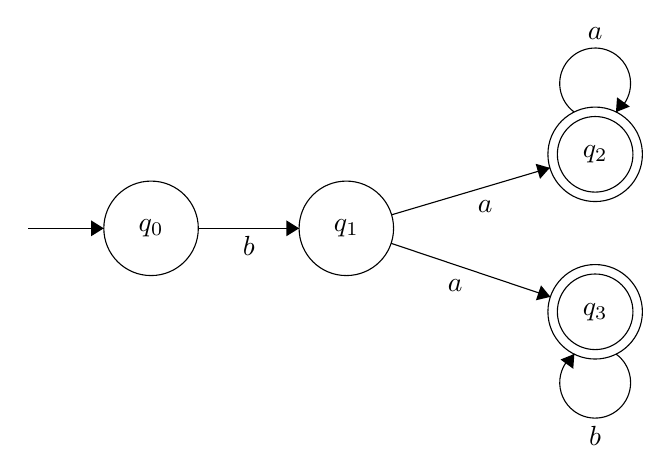
\begin{tikzpicture}[scale=0.2]
\tikzstyle{every node}+=[inner sep=0pt]
\draw [black] (12.4,-17.9) circle (3);
\draw (12.4,-17.9) node {$q_{0}$};
\draw [black] (24.8,-17.9) circle (3);
\draw (24.8,-17.9) node {$q_{1}$};
\draw [black] (40.6,-13.2) circle (3);
\draw (40.6,-13.2) node {$q_{2}$};
\draw [black] (40.6,-13.2) circle (2.4);
\draw [black] (40.6,-23.2) circle (3);
\draw (40.6,-23.2) node {$q_{3}$};
\draw [black] (40.6,-23.2) circle (2.4);
\draw [black] (39.277,-10.52) arc (234:-54:2.25);
\draw (40.6,-5.95) node [above] {$a$};
\fill [black] (41.92,-10.52) -- (42.8,-10.17) -- (41.99,-9.58);
\draw [black] (41.923,-25.88) arc (54:-234:2.25);
\draw (40.6,-30.45) node [below] {$b$};
\fill [black] (39.28,-25.88) -- (38.4,-26.23) -- (39.21,-26.82);
\draw [black] (27.68,-17.04) -- (37.72,-14.06);
\fill [black] (37.72,-14.06) -- (36.82,-13.8) -- (37.1,-14.76);
\draw (33.61,-16.11) node [below] {$a$};
\draw [black] (27.64,-18.85) -- (37.76,-22.25);
\fill [black] (37.76,-22.25) -- (37.16,-21.52) -- (36.84,-22.47);
\draw (31.72,-21.09) node [below] {$a$};
\draw [black] (4.6,-17.9) -- (9.4,-17.9);
\fill [black] (9.4,-17.9) -- (8.6,-17.4) -- (8.6,-18.4);
\draw [black] (15.4,-17.9) -- (21.8,-17.9);
\fill [black] (21.8,-17.9) -- (21,-17.4) -- (21,-18.4);
\draw (18.6,-18.4) node [below] {$b$};
\end{tikzpicture}
\end{center}

\newpage

We have to convert it to a one letter NFA - $A'$, which has a different language but it is known that $\Phi(A) = \Phi(A')$. Below you can see an example result of the conversion.

\begin{center}
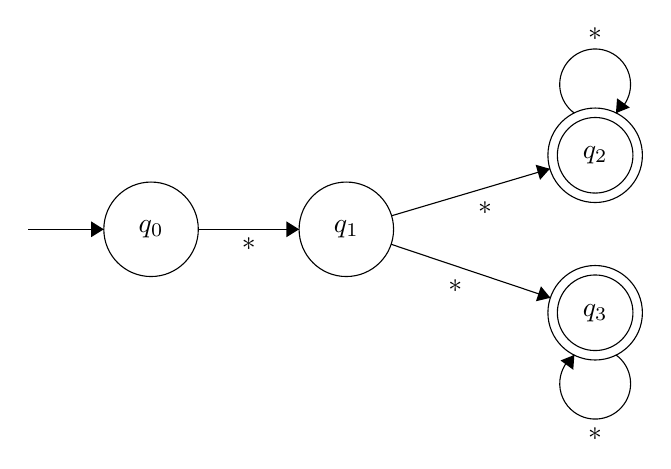
\begin{tikzpicture}[scale=0.2]
\tikzstyle{every node}+=[inner sep=0pt]
\draw [black] (12.4,-17.9) circle (3);
\draw (12.4,-17.9) node {$q_{0}$};
\draw [black] (24.8,-17.9) circle (3);
\draw (24.8,-17.9) node {$q_{1}$};
\draw [black] (40.6,-13.2) circle (3);
\draw (40.6,-13.2) node {$q_{2}$};
\draw [black] (40.6,-13.2) circle (2.4);
\draw [black] (40.6,-23.2) circle (3);
\draw (40.6,-23.2) node {$q_{3}$};
\draw [black] (40.6,-23.2) circle (2.4);
\draw [black] (39.277,-10.52) arc (234:-54:2.25);
\draw (40.6,-5.95) node [above] {$*$};
\fill [black] (41.92,-10.52) -- (42.8,-10.17) -- (41.99,-9.58);
\draw [black] (41.923,-25.88) arc (54:-234:2.25);
\draw (40.6,-30.45) node [below] {$*$};
\fill [black] (39.28,-25.88) -- (38.4,-26.23) -- (39.21,-26.82);
\draw [black] (27.68,-17.04) -- (37.72,-14.06);
\fill [black] (37.72,-14.06) -- (36.82,-13.8) -- (37.1,-14.76);
\draw (33.61,-16.11) node [below] {$*$};
\draw [black] (27.64,-18.85) -- (37.76,-22.25);
\fill [black] (37.76,-22.25) -- (37.16,-21.52) -- (36.84,-22.47);
\draw (31.72,-21.09) node [below] {$*$};
\draw [black] (4.6,-17.9) -- (9.4,-17.9);
\fill [black] (9.4,-17.9) -- (8.6,-17.4) -- (8.6,-18.4);
\draw [black] (15.4,-17.9) -- (21.8,-17.9);
\fill [black] (21.8,-17.9) -- (21,-17.4) -- (21,-18.4);
\draw (18.6,-18.4) node [below] {$*$};
\end{tikzpicture}
\end{center}

Next, we determinize our one letter NFA $A'$ to get a one letter deterministic finite automata (DFA) $A''$ using the powerset construction.

\begin{center}
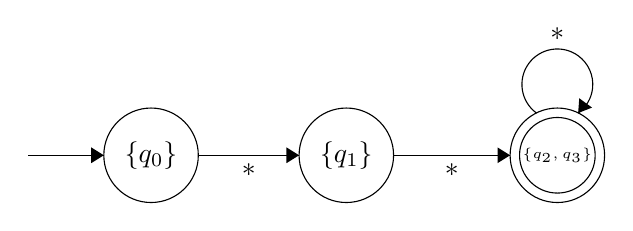
\begin{tikzpicture}[scale=0.2]
\tikzstyle{every node}+=[inner sep=0pt]
\draw [black] (12.4,-17.9) circle (3);
\draw (12.4,-17.9) node {$\{q_{0}\}$};
\draw [black] (24.8,-17.9) circle (3);
\draw (24.8,-17.9) node {$\{q_{1}\}$};
\draw [black] (38.2,-17.9) circle (3);
\draw (38.2,-17.9) node {\tiny{$\{q_{2}, q_{3}\}$}};
\draw [black] (38.2,-17.9) circle (2.4);
\draw [black] (27.8,-17.9) -- (35.2,-17.9);
\fill [black] (35.2,-17.9) -- (34.4,-17.4) -- (34.4,-18.4);
\draw (31.5,-18.4) node [below] {$*$};
\draw [black] (4.6,-17.9) -- (9.4,-17.9);
\fill [black] (9.4,-17.9) -- (8.6,-17.4) -- (8.6,-18.4);
\draw [black] (15.4,-17.9) -- (21.8,-17.9);
\fill [black] (21.8,-17.9) -- (21,-17.4) -- (21,-18.4);
\draw (18.6,-18.4) node [below] {$*$};
\draw [black] (36.877,-15.22) arc (234:-54:2.25);
\draw (38.2,-10.65) node [above] {$*$};
\fill [black] (39.52,-15.22) -- (40.4,-14.87) -- (39.59,-14.28);
\end{tikzpicture}
\end{center}

All one letter deterministic finite automata have handle and loop parts.


To illustrate how we create the formula from the one letter automaton, we choose a different example below.

\begin{center}
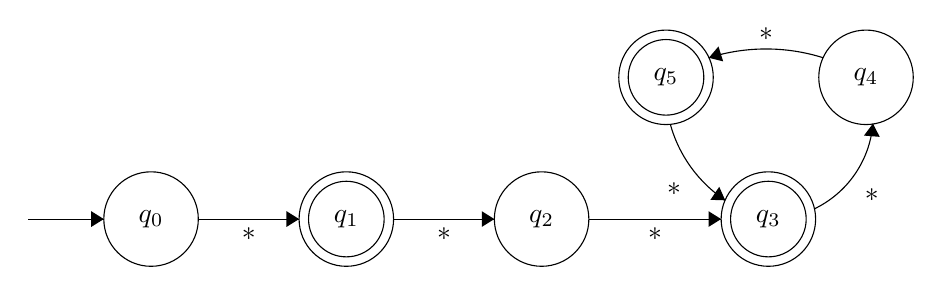
\begin{tikzpicture}[scale=0.2]
\tikzstyle{every node}+=[inner sep=0pt]
\draw [black] (12.4,-17.9) circle (3);
\draw (12.4,-17.9) node {$q_{0}$};
\draw [black] (24.8,-17.9) circle (3);
\draw (24.8,-17.9) node {$q_{1}$};
\draw [black] (24.8,-17.9) circle (2.4);
\draw [black] (37.2,-17.9) circle (3);
\draw (37.2,-17.9) node {$q_{2}$};
\draw [black] (51.6,-17.9) circle (3);
\draw (51.6,-17.9) node {$q_{3}$};
\draw [black] (51.6,-17.9) circle (2.4);
\draw [black] (57.8,-8.9) circle (3);
\draw (57.8,-8.9) node {$q_{4}$};
\draw [black] (45.1,-8.9) circle (3);
\draw (45.1,-8.9) node {$q_{5}$};
\draw [black] (45.1,-8.9) circle (2.4);
\draw [black] (27.8,-17.9) -- (34.2,-17.9);
\fill [black] (34.2,-17.9) -- (33.4,-17.4) -- (33.4,-18.4);
\draw (31,-18.4) node [below] {$*$};
\draw [black] (4.6,-17.9) -- (9.4,-17.9);
\fill [black] (9.4,-17.9) -- (8.6,-17.4) -- (8.6,-18.4);
\draw [black] (15.4,-17.9) -- (21.8,-17.9);
\fill [black] (21.8,-17.9) -- (21,-17.4) -- (21,-18.4);
\draw (18.6,-18.4) node [below] {$*$};
\draw [black] (40.2,-17.9) -- (48.6,-17.9);
\fill [black] (48.6,-17.9) -- (47.8,-17.4) -- (47.8,-18.4);
\draw (44.4,-18.4) node [below] {$*$};
\draw [black] (58.236,-11.842) arc (-4.61158:-64.51347:6.588);
\fill [black] (58.24,-11.84) -- (57.67,-12.6) -- (58.67,-12.68);
\draw (57.7,-16.4) node [right] {$*$};
\draw [black] (47.821,-7.656) arc (107.46434:72.53566:12.091);
\fill [black] (47.82,-7.66) -- (48.73,-7.89) -- (48.43,-6.94);
\draw (51.45,-6.6) node [above] {$*$};
\draw [black] (48.864,-16.708) arc (-123.64616:-164.67853:8.51);
\fill [black] (48.86,-16.71) -- (48.48,-15.85) -- (47.92,-16.68);
\draw (46.09,-15.99) node [left] {$*$};
\end{tikzpicture}
\end{center}

As we mentioned, it has two parts - the handle and the loop. Therefore, for our example, states $q_{0}, q_{1}, q_{2}, q_{3}$ and transitions between them are in the handle, states $q_{3}, q_{4}, q_{5}$ and transitions between them are in the loop.

\newpage
We mark the length of handle as $n$, the length of the part from the initial state to any state as $v$, the length of the loop as $k$, and $l$ represents cycling in the loop.
With the following algoritm we can determine the lengths of words in the language of the automaton. For every $q \in Q$ of an automaton $A$ we obtain $\Phi_q(A)$ as follows:

\[
  \Phi_q(A) =
  \begin{cases}
   |d| = v & \text{if $q$ in handle, $v < n$} \\
   |d| = v + k*l & \text{if $q$ in loop, $v \geq n$}
  \end{cases}
\]

Let us describe our implementation in detail. The input of our algorithm is a one letter deterministic finite automaton and the output is pthe formula of lengths of words of the language of this automaton. The implemementation in following pseudocode presented below works with the automanon using the following data structures. There is aut, which is structure which holds states of an automaton as an array of pointers, the initial state is represeted as the first item in this array. We have a record called state which contains truth value whether this state is final or not, and pointer to the next state, if any. We have two counters - to count the length of the part from the initial state to any state and to count the length of the loop. Also, we use an array to save states in the loop. After we find any final state, we put it to this array and we put all following states here too. We check if there is any state in this array twice - which means an infinite cycling and therefore, no loop. We count the length of the part from the initial state to any final state. Then we count the length of the loop and finally we print the formula of the lengths of the words in the language of the automata.

\newpage
\begin{lstlisting}
first = aut.states[0];
for state in aut.states:
    loop_states = {};
    v = 0, loop = 1; s = first;
    is_loop = true, in_loop = false;
    
    while (true) {
	if (loop_states.contains(s) && s == state)) {
	    break;
	}
	
	if (s == NULL) {
            is_loop = false;
            break;
        }
	
	if (s == state) {
            in_loop = true;
            if (s.is_final) {
                print("d = %d", v);
            }
	}
	
	if (in_loop) {
	     if (loop_states.contains(s)) {
	        is_loop = false;
	        break;
	    }
	    loop_states.add(s);
	    loop++;
	} else {
	    v++;
	}
	
	s = s.next;
    }

    if (is_loop) print("d = %d + %d * l", v, loop);
\end{lstlisting}


With computed lengths and especially, the final artimetic formula, we can safely aproximate the emptiness test. SMT solver processes our aritmetic formula $SAT(\Phi(A) \wedge \Phi(B))$ and we are finally able to decide about the emptiness of intersection of automata by checking if the formula is satisfiable or not. If it is not, then intersection is empty, otherwise we don't know anything useful (as typical fact for safe approximation).
We implemented our algoritm in Java. We used BRICS library \footnote{\url{http://www.brics.dk/automaton/}} for automaton operations like determinization. As a SMT solver, we chose open source solver called Alt-Ergo \footnote{\url{http://alt-ergo.lri.fr/}}.
\chapter{Conclusion}
Our aim has been to implement basic version of algorithm to decide about emptiness of automata intersection. As we see, in the basic version, we have useful information about the emptiness only if the intersection is satisfiable - if it is not, we know nothing. As we mentioned in the Introduction, possibly the next work to solve this problem more efficiently would be based on tightly interconnection of product construction with the lengths of words and / or Parikh images.
